\documentclass{article}
\usepackage{graphicx}

\title{Project 1 Answers}
\date{2020-06-29}
\author{Edward Wang, Atishay Mitra, Kyle Love}

\begin{document}
\maketitle

\section{Part 1}
a. Since the agent can only observe its 4 adjacent cells, it will choose to move to the east in the first step since the cell to the east is unblocked and is currently the first step on the shortest path to the target state. After the agent would move to position E3, it would observe that the north and east cells are blocked and adjust its path. 

b. In a finite gridworld, there will be a limited number of cells which the agent must check and therefore the time required to find the path or conclude that a path to the target does not exist will be finite. The time it takes to search is linked to the finite number of cells. In contrast, a search algorithm applied on an infinite, constantly expanding gridworld could take an infinite amount of time to conclude whether an agent can reach its target or not.

The number of moves the agent can make is bounded from above by the number of unblocked cells squared because if an adjacent cell is blocked then the agent will backtrack to the same cell at most one time meaning that they will have visited the cell at most two times within the algorithm before either realizing that there is another path or that there is no path at all to the target. 

\section{Part 2}

\section{Part 3}
To test and compare the performance of Repeated Forward A* against Repeated Backward A*, we conducted runs of the algorithms once on each of the fifty grid worlds generated. Firstly, we applied Forward A*, randomly choosing nodes for both the goal and start, then swapped those same nodes and ran it again to simulate Backward A*. We then took the resulting values for the number of expanded nodes and compared them to determine their efficiency. Below are example runs, and the percent difference between the different algorithms in terms of nodes expanded.
\begin{figure}
	\caption{Example Forward A* path}
	\centering
	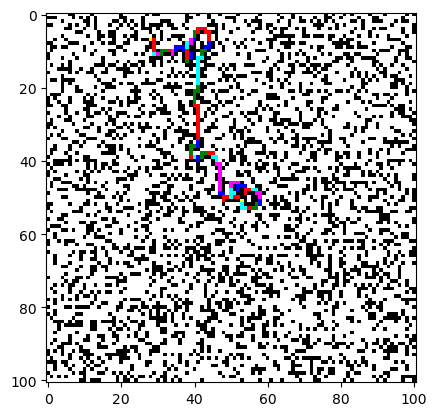
\includegraphics[scale=0.75]{visF}
\end{figure}
\begin{figure}
	\caption{Example Backward A* path}
	\centering
	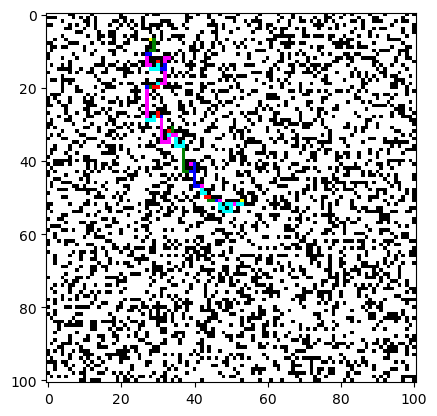
\includegraphics[scale=0.75]{visB}
\end{figure}
\begin{center}
	\begin{tabular}{|c|c|c|}
		\hline
		Percent Difference & Forward A* & Backward A* \\
		\hline
		60.6\% & 816 & 508 \\
		62.8\% & 482 & 296 \\
		-20.8\% & 19 & 24 \\
		-44.2\% & 829 & 1487 \\
		12.8\% & 2024 & 1793 \\
		-36.5\% & 453 & 713 \\
		246\% & 1974 & 517 \\
		56.4\% & 341 & 218 \\
		20.6\% & 262 & 330 \\
		-42.2\% & 1783 & 3086 \\
		\hline
	\end{tabular}
\end{center}

On average, we determined that Forward A* had a runtime 19.66\% lesser that that of Backward A* for the same grids and nodes. Overall, the data seems to suggest that Forward A* is more efficient that Backward A*. However, it is also important to note that, in theory, the two algorithms should have similar performance, given that the obstacles/blocked nodes should hypothetically be spaced randomly. The results we have found are may be largely due to our small sample size. As such, it is hard to conclude off of our data that Forward A* is in fact slower than Backward A*.
\section{Part 4}
\subsection{Manhattan distances}
The manhattan distance is calculated with the following formula
\begin{equation}
	h(s) = |X_s - X_{goal}| + |Y_s - Y_{goal}|
\end{equation}
To be considered a consistent heuristic, it must prove true for the following formula
\begin{equation}
	h(s) <= h(s')+c(s,a,s')
\end{equation}
 We substitute all instances of h(s) and h(s') with the corresponding manhattan distance definition.
\begin{equation}
	|X_s - X_{goal}| + |Y_s - Y_{goal}| <= |X_s' - X_{goal}| + |Y_s' - Y_{goal}| + c(s,a,s')
\end{equation}
Then simplify
\begin{equation}
	|X_s - X_{goal}| + |Y_s - Y_{goal}| - |X_s' - X_{goal}| + |Y_s' - Y_{goal}| <= c(s,a,s')
\end{equation}
Say s and s' are neighboring cells, s' being the immediate successor of the initial state. Furthermore, let us say that s' is vertically adjacent to s. Hence, the following proves true.
\begin{equation}
	|X_s - X_{goal}| - |X_s' - X_{goal}| = 0	
\end{equation}
\begin{equation} 
	|Y_s - Y_{goal}| - |Y_s' - Y_{goal}| = 1
\end{equation}
\begin{equation} 
	|Y_s - Y_s'| = 1
\end{equation}
\begin{equation} 
	|Y_s - Y_{goal}| - |Y_s' - Y_{goal}| = c(s,a,s')
\end{equation}
\begin{equation} 
	h(s) - h(s') = |Y_s - Y_{goal}| - |Y_s' - Y_{goal}|
\end{equation}
Then, given the following inequality
\begin{equation}
	|A| - |B| <= |A-B|
\end{equation}
we say
\begin{equation}
	h(s) - h(s') <= |(Y_s - Y_{goal}) - (Y_s' - Y_{goal})|
		= 1
		= c(s,a,s')
\end{equation}
Therefore, manhattan distances can be said to be consistent heuristics.
\subsection{Adaptive A*}
To prove conclusively that Adaptive A* leaves heuristics consistent over iterations, we must prove it's validity for the following three cases
\subsubsection{In the case both s and s' are expanded}
The new heuristics for both of the nodes are as follows
\begin{equation}
h_{new}(s) = g(s_{goal})-g(s)
\end{equation}
\begin{equation}
h_{new}(s') = g(s_{goal})-g(s')
\end{equation}
We then substitute them into the consistency inequality like so
\begin{equation}
h_{new}(s) <= h_{new}(s')+c(s,a,s')
\end{equation}
\begin{equation}
g(s_{goal}) - g(s) <= g(s_{goal}) - g(s') + c(s,a,s')
\end{equation}
\begin{equation}
g(s') <= g(s) + c(s,a,s')
\end{equation}
Using the above equation, we can conclusively state that the heuristic remains consistent because the algorithm calculates the g value of the successor state based off of the g value of its predecessor with the cost to transition added, so the inequality will never be false.
\subsubsection{In the case s, but not s' is expanded}
The consistency inequality we want to prove in this case is as follows
\begin{equation}
h_{new}(s) <= h(s') + c(s,a,s')
\end{equation}
Firstly, considering that case 1 holds true, we can similarly say that case 2 holds true, because the inequality would still be valid if the node were to be expanded. Nothing changed with regards to the situation, only the amount of information we have has changed. 
Furthermore,
\begin{equation}
f(s) <= f(s')
\end{equation}
because the algorithm prioritizes the smallest f-value to expand nodes. Therefore, if we substitute into the equation above as follows, splitting the f-value into h+g values,
\begin{equation}
	h_{new}(s) + g(s) <= h(s') + c(s,a,s') + g(s)
\end{equation}
we find that 
\begin{equation}
h_{new}(s) <= h(s') + c(s,a,s')
\end{equation}
proving the inequality true
\subsubsection{In the case neither are expanded}
Unlike the other cases, the adaptive A* algorithm modifies neither s or s', so considering the fact that the consistency inequality should hold true in normal A*, we can conclude that this case holds true as well.
\section{Part 5}
To test Adaptive A* against Forward A*, we underwent a similar process to the Backward A* vs Forward A* trials, comparing the Adaptive A* algorithm for the same nodes as the initial Forward A* trials to determine which of them was the more efficient. A sample of ten of the trials is shown below.

\begin{center}
	\begin{tabular}{|c|c|c|}
		\hline
		Percent Difference & Forward A* & Adaptive A* \\
		\hline
		0\% & 816 & 816 \\
		0\% & 482 & 482 \\
		0\% & 19 & 19 \\
		0\% & 829 & 829 \\
		0\% & 2024 & 2024 \\
		0\% & 453 & 453 \\
		0\% & 1974 & 1974 \\
		0\% & 341 & 341 \\
		0\% & 262 & 262 \\
		0\% & 1783 & 1783 \\
		\hline
	\end{tabular}
\end{center}
As can be seen, in the majority of cases, Adaptive A* seems to perform almost exactly the same as 

\section{Part 6}

\end{document}
